\documentclass[handout]{beamer}      % print handout
%\documentclass[notes]{beamer}       % print frame + notes
%\documentclass[notes=only]{beamer}   % only notes
%\documentclass{beamer}              % only frames
\usetheme{DSL}
%\useouterthen{DSL}
\usepackage{url}
\usepackage{hyperref}
\usepackage{textcomp}
\usepackage{algorithm}
\usepackage{algpseudocode}
\usepackage{listings}
\lstset{
  language=C++,
  breaklines=true,
  tabsize=2,
  showspaces=false,
  %stepnumber=10
  basicstyle=\scriptsize
}
\algrenewcommand\alglinenumber[1]{\scriptsize #1:}


\setbeamertemplate{bibliography item}{[\theenumiv]}
%\setbeamertemplate{footline}{\hfill\insertframenumber/\inserttotalframenumber}
\setbeamertemplate{caption}[numbered]
% allow "(cont.)" to be used
\setbeamertemplate{frametitle continuation}[from second]

\title[Building Chatbot]{Building Your Own Chatbot}

\author[Gou \and Ghose]
{%
  \scriptsize
  \texorpdfstring{
    \begin{columns}%[onlytextwidth]
      \column{.3\linewidth}
      \centering
      Yingzhi Gou\\
      \href{mailto:yg452@uowmail.edu.au}{yg452@uowmail.edu.au}
      \column{.3\linewidth}
      \centering
      Aditya Ghose\\
      \href{mailto:aditya@uow.edu.au}{aditya@uow.edu.au}
    \end{columns}
  }
  {Yingzhi Gou \and Aditya Ghose}
}
\institute[DSL]{Decision Systems Lab\\School of Computing and Information Science\\University of Wollongong, Australia}
\date{15 June 2018}

\begin{document}
%%  LOGO ========================
\addtobeamertemplate{headline}{}
{%
\begin{flushright}
%\begin{tikzpicture}[remember picture,overlay]
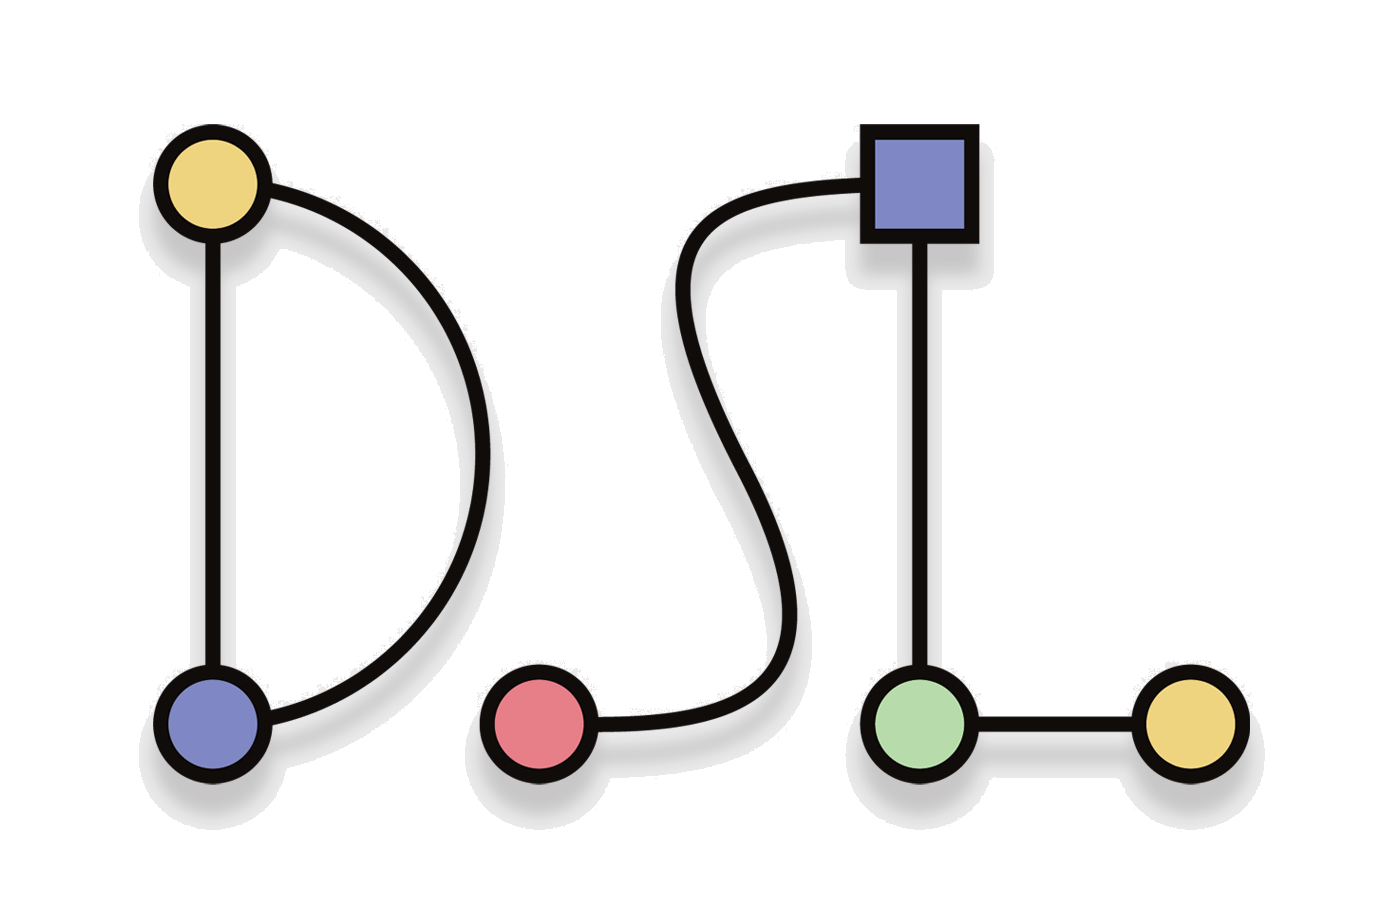
\includegraphics[width=2cm,keepaspectratio]{DSL_new_logo}
%\end{tikzpicture}
\end{flushright}
\vskip -0.5cm
} 


\frame{\titlepage}

\section*{outline}
\begin{frame}
  \frametitle{Outline}
  \tableofcontents
\end{frame}

\section{Introducing the Chatbots}

\begin{frame}
    \frametitle{Introducing the Chatbots}
    \begin{itemize}
        \item TWO chatbots are here today
        \item You can find and talk to them on \href{https://telegram.org/}{Telegram}.
        \item Mary (\href{https://t.me/MaryDSLBot}{@MaryDSLBot}), and
        \item Dora (\href{https://t.me/DoraDSLBot}{@DoraDSLBot})
    \end{itemize}
\end{frame}

\section{DeepQA - A Neural Conversational Model}

\begin{frame}
    \frametitle{DeepQA - A Neural Conversational Model}
    \begin{itemize}
        \item A Sequence to sequence (seq2seq) model
        \item Being successfully used in machine translation
        \item Also used to create chatbots such as the Google chatbot in 2015
    \end{itemize}
    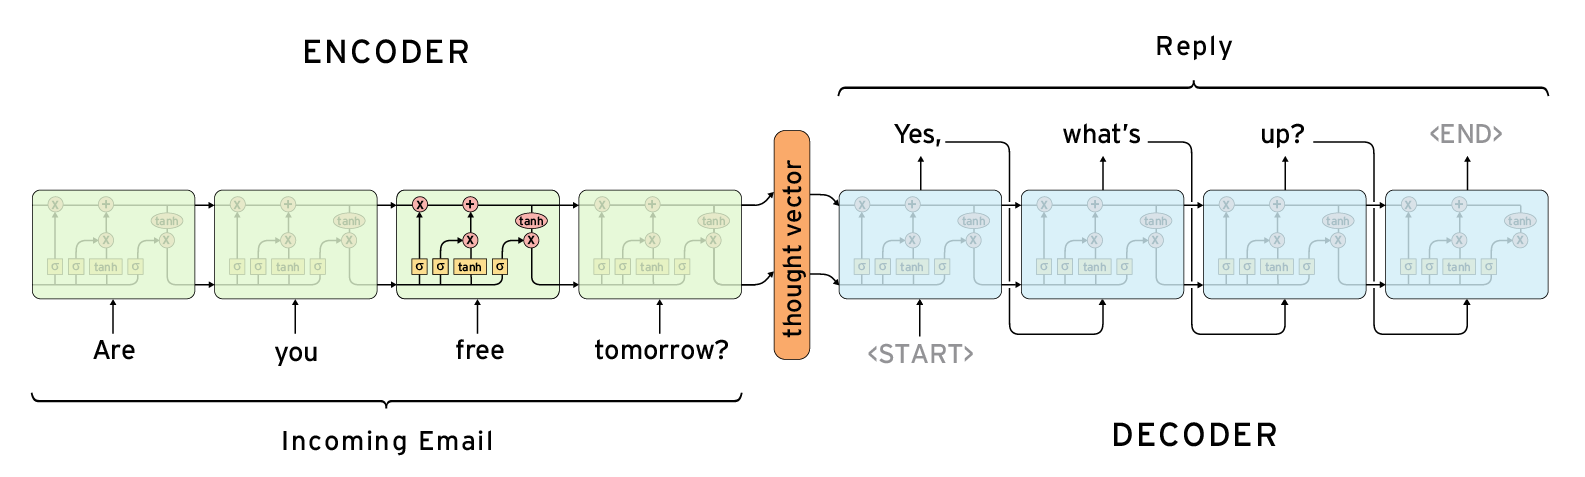
\includegraphics[width=\textwidth]{image01.png}\footnote{Image source: \href{http://www.wildml.com/2016/04/deep-learning-for-chatbots-part-1-introduction/}{Deep Learning for chatbots part 1}}
\end{frame}

\begin{frame}

\end{frame}
\end{document}
